\documentclass[14pt, a4paper,oneside]{extarticle}
\usepackage[T1,T2A]{fontenc}
\usepackage[utf8]{inputenc}
\usepackage[russian]{babel}
\usepackage{epstopdf}
\usepackage{verbatim}
\usepackage[linesnumbered,boxed]{algorithm2e}
\usepackage[]{graphicx}
\usepackage{setspace}

\usepackage{indentfirst}
\usepackage{hyperref} %url

\usepackage{amsmath} 
 \setcounter{tocdepth}{2} 
\usepackage{floatrow}
% Table float box with bottom caption, box width adjusted to content
\newfloatcommand{capbtabbox}{table}[][\FBwidth]

\onehalfspacing

%\graphicspath{{image/}}
\usepackage[left=2cm,right=2cm,bottom=3cm,top=2cm]{geometry}
\bibliographystyle{unsrt}
\SetKwProg{Op}{Operator}{}{}
\SetKwProg{Func}{Function}{}{}
\SetAlgoNlRelativeSize{0}
\author{Швецов Денис}
\title{Реферат по английскому}
\begin{document}
\thispagestyle{empty}

	\thispagestyle{empty}
	
	\begin{center}
		\ \vspace{-0.5cm}
		
		
\includegraphics[width=0.5\textwidth]{msu}\\
		{Московский государственный университет имени М.В. Ломоносова}\\
		Факультет вычислительной математики и кибернетики\\
		Кафедра автоматизации систем вычислительных комплексов
		
		\vspace{2.5cm}
		
		{\Large ШВЕЦОВ Денис Андреевич}
		
		\vspace{1cm}
		
		{\Large\bfseries
			Алгоритмы управления перегрузками в центрах обработки данных\\}
		
		\vspace{2cm}
		
		{\large РЕФЕРАТ}
	\end{center}
	\vfill
	\begin{center}
		Москва, 2017
	\end{center}
	\vspace{1cm}
	\enlargethispage{4\baselineskip}

\section{Введение}

На сегодняшний день центры обработки данных являются важнейшей частью инфраструктуры организаций предоставляющие всевозможные он-лайн сервисы для своих клиентов, например, веб-поиск, торговые площадки, рекомендательные системы. Качество работы этих сервисов напрямую влияет на количество заинтересованных пользователей и следственно на доход. 

Приложения он-лайн сервисов должны работать в реальном времени~--- пользователь вводит запрос в веб-браузере и ожидает незамедлительного отклика (время отклика не должно превышать 300 миллисекунд). 
Так же приложения работают с большими объемами данных (например, весь веб-индекс) для формирования ответа на запрос. Обычно эти данных распределены между тысячами сервером и каждый запрос попадает на все сервера.

Высокие нагрузки на центры обработки данных и жесткие требования приложений порождают жесткие требования на сети в центрах обработки данных. Работа приложений в реальном времени требует низких задержек в сети и устойчивости к разрывам. Также поскольку приложениям надо постоянно обновлять внутренние структуры данных сети должны иметь высокую пропускную способность для длительных потоков. При этом, несмотря на предъявленные требования, в сетях центров обработки данных зачастую используется дешевое сетевое оборудование, например, ToR (Top of the rack) коммутатор, который соединяет между собой сервера в стойке, имеет 48 портом скоростью 1 гигабит в секунду.

В условиях сетей центров обработки данных TCP протокол не достаточно хорошо справляется с поставленными требованиями~\cite{dctcp}, поэтому ведутся работы по разработке протоколов управления перегрузками в центрах обработки данных.
Cуществуют подходы, в которых используются возможности протокола TCP, такие как ECN метка~\cite{dctp, d2tcp}, при этом остальные функции протокола остаются нетронутыми.
Параллельно с этим существуют работы, в которых, разрабатывают протоколы не совместимые с TCP~\cite{d3tcp}, например, Facebook разработала свой протокол управления перегрузками поверх UDP~\cite{facebook}.

\newpage

\section{Центры обработки данных}
\subsection{Приложения центров обработки данных}

На сегодняшний день крупномасштабные приложения в центрах обработки данных используют разработаны в соответствии с подходом разделение/агрегация (см. рисунок % partition/aggreagate pattern
Запрос с уровней, расположенных наверху, делится на части и передаются на нижний уровень обрабатывающем процессам. Ответ от этих обрабатывающих процессов агрегируется для получения результирующего ответа. Такой подход используется даже в таких сервисах обработки данных как MapReduce и  Dryad. % Может быть и тут ссылки вставаить

Интерактивная природа веб-приложений означает, что задержка это значимый параметр. Приложения обычно имеют ограничения в 200-300 миллисекунд для того, чтобы завершить свои вычисления и вернуть ответ пользователю~\cite{sla}. Это ограничение ведет к тому приводят к ограничениям на задержку на каждом уровне иерархии центров обработки данных. Эти ограничения означают, что сетевые потоки, которые несут в себе запросы и ответы к узлам и от них, имеет директивные интервалы выполнения, и если какой-то узел не уложился в свой директивный интервал, вычисления продолжаются без его ответа, что снижает качество результата, не говоря уже о бесполезном использовании пропускной способности сети.

\subsection{Сетевая нагрузка в центрах обработки данных}
Были проведены исследования о том, какой трафик существует в центрах обработки данных~\cite{dctcp}, были выделены три различных типов трафика:
\begin{enumerate}
\item трафик запросов
\item трафик коротких сообщений, который координирует активность в центре обработки данных
\item фоновый трафик, который передает большие объемы данных между серверами для того, чтобы приложения поддерживали внутренние структуры в актуальном состоянии и выдали ответы высокого качества.
\end{enumerate}

\paragraph{Трафик запросов.}
Трафик запросов использует модель разделения агрегации и состоит из очень коротких потоков, критичных к задержке. Агретор высшего уровня разделяет запрос на большое количество агрегаторов среднего уровня, которые в свою очередь деляет каждый запрос на 43 других сервера, находящийся в той же самой стойке. Размеры трафика запросов достаточно постоянный~--- 1,6 килобайт для запросов и 1,6-2 килбоайта для ответов.
% Можно еще припихнуть картинку про распределение времени между двумя запросами

\paragraph{Фоновый трафик.}
\begin{figure}
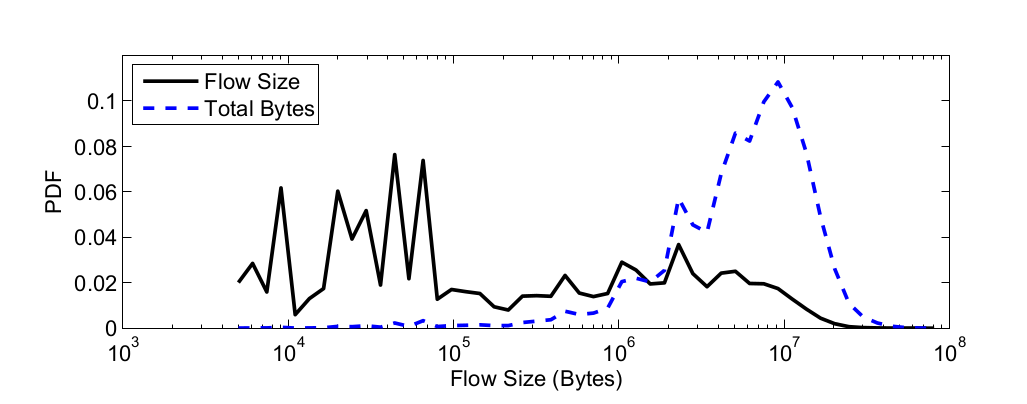
\includegraphics[width=\linewidth]{pdf_of_flow_size.png}
\caption{Плотность вероятности размера потока для фонового трафика. Плотность вероятности общего количество данных показывает вероятность того, что случайно выбранный байт будет принадлежать потоку данного размера.}
\label{pdf_of_flow_size}
\end{figure}

Параллельно с трафиком запросов существует фоновый трафик, состоящий и из больших и из маленьких потоков. % Плостность распредления потоков
На рисунке~\ref{pdf_of_flow_size} видно, что большинство фоновых потоков имеет маленький размер, но большинство данных в фоновом трафике принадлежит большим потокам.
%TODO Дописать эту часть

\subsection{Проблемы сетей в центрах обработки данных}

Большинство коммутаторов в центрах обработки данных это \emph{коммутаторы с разделяемой памятью}, использующие статического мультиплексирования с помощью буфера пакетов доступного для всех портов коммутатора. Пакет прибывает на интерфейс и сохраняется в высокоскоростную память разделенную между всеми интерфейсами. Устройство управления памятью динамически выделяет для пакета память. Устройство управления памятью старается дать интерфейсу столько памяти, сколько ему необходимо, динамически настраивая максимальный объем памяти, который может использовать любой интерфейс.
Если пакет должен быть поставлен в очередь на отправку на некоторый интерфейс, но этот интерфейс достиг максимума выделенной ему памяти или истощился сам пул свободной разделяемой памяти, тогда пакет будет отброшен. Создание разделяемой памяти большого объема очень дорогой процесс, поэтому большинство дешевых коммутаторов имеют \emph{маленький буфер пакетов}. Этот маленький буфер пакетов является причиной трех специфичных проблем, которые описаны далее.


\newpage
\begin{thebibliography}{9}
\addcontentsline{toc}{section}{\bibname}

\bibitem {dctcp}
Alizadeh M., Greenberg A., Maltz
 D.A., Padhye J., Patel P., Prabhakar B., 
Sengupta S., and Sridharan M. Data Center TCP (DCTCP) // ACM SIGCOMM 
Computer Communication Review -
 SIGCOMM '10, Volume 40 Issue 4. Oct. 
2010. Pp. 63
-74.

\bibitem {d3tcp}
Wilson C., Ballani H., Karagiannis T., Rowtron
 A. Better never than late: meeting 
deadlines in datacenter networks // ACM SIGCOMM Computer Communication 
Review 
- SIGCOMM '11 Volume 41 Issue 4. Aug. 2011. Pp. 50
-61. 

\bibitem {d2tcp}
Vamanan B., Hasan J., Vijaykumar T.N. Deadline
-aware datacenter tcp (D2TCP) 
// Proceedi
ngs of the ACM SIGCOMM 2012 conference on Applications, 
technologies, architectures, and protocols for computer communication. Aug. 
2012. Pp. 115
-126. 

\bibitem {facebook}
Nishtala R. et al. Scaling Memcache at Facebook //nsdi. – 2013. – Т. 13. – С. 385-398.

\bibitem {sla}
DeCandia G. et al. Dynamo: amazon's highly available key-value store //ACM SIGOPS operating systems review. – 2007. – Т. 41. – №. 6. – С. 205-220.

\end{thebibliography}

\end{document}